\section{Overview}\label{sec:overview}

\begin{figure*}[t]
  \centering
  

\tikzset{every picture/.style={line width=0.75pt}} %set default line width to 0.75pt        

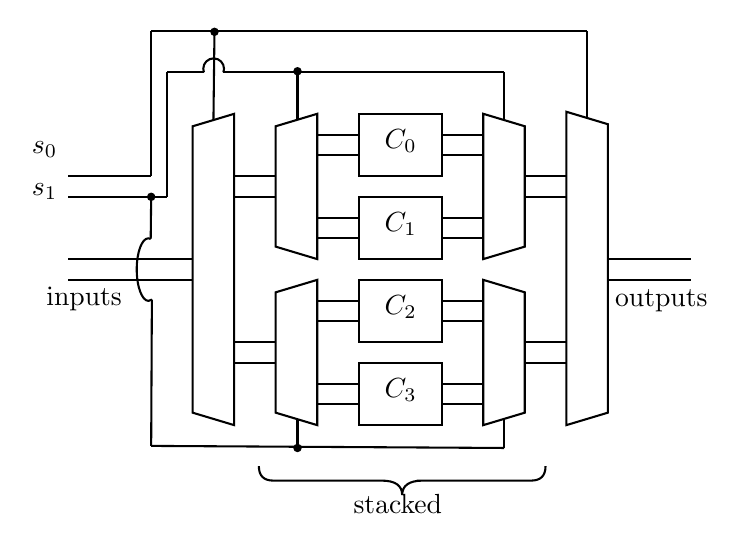
\begin{tikzpicture}[x=0.75pt,y=0.75pt,yscale=-1,xscale=1]
%uncomment if require: \path (0,300); %set diagram left start at 0, and has height of 300

%Shape: Rectangle [id:dp5849077965847459] 
\draw   (330,100) -- (370,100) -- (370,130) -- (330,130) -- cycle ;
%Shape: Rectangle [id:dp07483417235317913] 
\draw   (330,140) -- (370,140) -- (370,170) -- (330,170) -- cycle ;
%Shape: Rectangle [id:dp4166376635287651] 
\draw   (330,180) -- (370,180) -- (370,210) -- (330,210) -- cycle ;
%Shape: Rectangle [id:dp8948354008474025] 
\draw   (330,220) -- (370,220) -- (370,250) -- (330,250) -- cycle ;
%Shape: Trapezoid [id:dp4540566847726426] 
\draw   (310,170) -- (290,164) -- (290,106) -- (310,100) -- cycle ;
%Straight Lines [id:da8956407127966497] 
\draw    (310,120) -- (330,120) ;
%Straight Lines [id:da9777100515836975] 
\draw    (310,110) -- (330,110) ;
%Straight Lines [id:da7425735986407294] 
\draw    (310,160) -- (330,160) ;
%Straight Lines [id:da11610382072678038] 
\draw    (310,150) -- (330,150) ;
%Straight Lines [id:da27169680424513776] 
\draw    (310,200) -- (330,200) ;
%Straight Lines [id:da727422130795774] 
\draw    (310,190) -- (330,190) ;
%Straight Lines [id:da209391042823457] 
\draw    (310,240) -- (330,240) ;
%Straight Lines [id:da44658343194865846] 
\draw    (310,230) -- (330,230) ;
%Straight Lines [id:da6142780982072071] 
\draw    (370,120) -- (390,120) ;
%Straight Lines [id:da6226887597311331] 
\draw    (370,110) -- (390,110) ;
%Straight Lines [id:da2664739221488589] 
\draw    (370,160) -- (390,160) ;
%Straight Lines [id:da026874100929834] 
\draw    (370,150) -- (390,150) ;
%Straight Lines [id:da9856263025895075] 
\draw    (370,200) -- (390,200) ;
%Straight Lines [id:da8016895233324299] 
\draw    (370,190) -- (390,190) ;
%Straight Lines [id:da013651076135336226] 
\draw    (370,240) -- (390,240) ;
%Straight Lines [id:da06626402429808187] 
\draw    (370,230) -- (390,230) ;
%Shape: Trapezoid [id:dp4574780651842486] 
\draw   (430,99) -- (450,105) -- (450,244) -- (430,250) -- cycle ;
%Straight Lines [id:da14149950401750877] 
\draw    (190,180) -- (250,180) ;
%Straight Lines [id:da2825534237984859] 
\draw    (190,170) -- (250,170) ;
%Straight Lines [id:da26233199494209225] 
\draw    (450,180) -- (490,180) ;
%Straight Lines [id:da15777944558688706] 
\draw    (450,170) -- (490,170) ;
%Straight Lines [id:da683223825833436] 
\draw    (190,140) -- (237.7,140) ;
%Straight Lines [id:da4217351698536934] 
\draw    (190,130) -- (230,130) ;
%Straight Lines [id:da9042212392696709] 
\draw    (260,103) -- (260.5,60.5) ;
%Shape: Trapezoid [id:dp5029111964216062] 
\draw   (310,250) -- (290,244) -- (290,186) -- (310,180) -- cycle ;
%Shape: Trapezoid [id:dp11848362887830954] 
\draw   (270,250) -- (250,244) -- (250,106) -- (270,100) -- cycle ;
%Shape: Trapezoid [id:dp4334595235977725] 
\draw   (390,100) -- (410,106) -- (410,164) -- (390,170) -- cycle ;
%Shape: Trapezoid [id:dp47262860257177874] 
\draw   (390,180) -- (410,186) -- (410,244) -- (390,250) -- cycle ;
%Straight Lines [id:da06426061609854339] 
\draw    (270,140) -- (290,140) ;
%Straight Lines [id:da21518984477524328] 
\draw    (270,130) -- (290,130) ;
%Straight Lines [id:da2852878452340667] 
\draw    (270,220) -- (290,220) ;
%Straight Lines [id:da83134608540614] 
\draw    (270,210) -- (290,210) ;
%Straight Lines [id:da4494574594480205] 
\draw    (410,220) -- (430,220) ;
%Straight Lines [id:da1998395845247215] 
\draw    (410,210) -- (430,210) ;
%Straight Lines [id:da8502911411231295] 
\draw    (410,140) -- (430,140) ;
%Straight Lines [id:da7117267186463382] 
\draw    (410,130) -- (430,130) ;
%Straight Lines [id:da17708779177622558] 
\draw    (230,60) -- (230,130) ;
%Straight Lines [id:da9403642725033405] 
\draw    (440,60) -- (413.64,60) -- (230,60) ;
%Straight Lines [id:da7042497085459944] 
\draw    (440,102) -- (440,60) ;
%Straight Lines [id:da02805679708561859] 
\draw    (237.7,80) -- (237.7,140) ;
%Straight Lines [id:da07817997121553377] 
\draw    (255.4,80) -- (237.7,80) ;
%Shape: Arc [id:dp44239178337134166] 
\draw  [draw opacity=0] (255.4,80) .. controls (255.21,79.47) and (255.1,78.89) .. (255.1,78.29) .. controls (255.1,75.53) and (257.34,73.29) .. (260.1,73.29) .. controls (262.86,73.29) and (265.1,75.53) .. (265.1,78.29) .. controls (265.1,78.89) and (264.99,79.47) .. (264.8,80) -- (260.1,78.29) -- cycle ; \draw   (255.4,80) .. controls (255.21,79.47) and (255.1,78.89) .. (255.1,78.29) .. controls (255.1,75.53) and (257.34,73.29) .. (260.1,73.29) .. controls (262.86,73.29) and (265.1,75.53) .. (265.1,78.29) .. controls (265.1,78.89) and (264.99,79.47) .. (264.8,80) ;
%Straight Lines [id:da536984199276638] 
\draw    (400,80) -- (264.8,80) ;
%Straight Lines [id:da9432174552358485] 
\draw    (400,103) -- (400,80) ;
%Straight Lines [id:da35579058464398416] 
\draw    (300.5,261) -- (300.5,247) ;
%Straight Lines [id:da2050986286068066] 
\draw    (400,261) -- (400,247) ;
%Straight Lines [id:da19791404796609613] 
\draw    (400,261) -- (230,260) ;
%Straight Lines [id:da09964823261578626] 
\draw    (230,140) -- (229.77,160.29) ;
%Shape: Arc [id:dp5324078769456657] 
\draw  [draw opacity=0] (230.34,189.49) .. controls (229.83,189.91) and (229.28,190.13) .. (228.72,190.13) .. controls (225.61,190.14) and (223.07,183.4) .. (223.04,175.07) .. controls (223.02,166.75) and (225.52,159.99) .. (228.64,159.98) .. controls (229.03,159.98) and (229.41,160.09) .. (229.77,160.29) -- (228.68,175.06) -- cycle ; \draw   (230.34,189.49) .. controls (229.83,189.91) and (229.28,190.13) .. (228.72,190.13) .. controls (225.61,190.14) and (223.07,183.4) .. (223.04,175.07) .. controls (223.02,166.75) and (225.52,159.99) .. (228.64,159.98) .. controls (229.03,159.98) and (229.41,160.09) .. (229.77,160.29) ;
%Straight Lines [id:da5048114542451922] 
\draw    (230.34,189.49) -- (230,260) ;
%Shape: Circle [id:dp9836025716711807] 
\draw  [fill={rgb, 255:red, 0; green, 0; blue, 0 }  ,fill opacity=1 ] (228.5,140) .. controls (228.5,139.17) and (229.17,138.5) .. (230,138.5) .. controls (230.83,138.5) and (231.5,139.17) .. (231.5,140) .. controls (231.5,140.83) and (230.83,141.5) .. (230,141.5) .. controls (229.17,141.5) and (228.5,140.83) .. (228.5,140) -- cycle ;
%Shape: Circle [id:dp135415838144737] 
\draw  [fill={rgb, 255:red, 0; green, 0; blue, 0 }  ,fill opacity=1 ] (299,261) .. controls (299,260.17) and (299.67,259.5) .. (300.5,259.5) .. controls (301.33,259.5) and (302,260.17) .. (302,261) .. controls (302,261.83) and (301.33,262.5) .. (300.5,262.5) .. controls (299.67,262.5) and (299,261.83) .. (299,261) -- cycle ;
%Shape: Circle [id:dp8636057586751603] 
\draw  [fill={rgb, 255:red, 0; green, 0; blue, 0 }  ,fill opacity=1 ] (299,79.5) .. controls (299,78.67) and (299.67,78) .. (300.5,78) .. controls (301.33,78) and (302,78.67) .. (302,79.5) .. controls (302,80.33) and (301.33,81) .. (300.5,81) .. controls (299.67,81) and (299,80.33) .. (299,79.5) -- cycle ;
%Straight Lines [id:da041429861674520674] 
\draw    (300.5,103) -- (300.5,81) ;
%Shape: Circle [id:dp005195803815501665] 
\draw  [fill={rgb, 255:red, 0; green, 0; blue, 0 }  ,fill opacity=1 ] (259,60.5) .. controls (259,59.67) and (259.67,59) .. (260.5,59) .. controls (261.33,59) and (262,59.67) .. (262,60.5) .. controls (262,61.33) and (261.33,62) .. (260.5,62) .. controls (259.67,62) and (259,61.33) .. (259,60.5) -- cycle ;
%Shape: Brace [id:dp3838971664751233] 
\draw   (281.88,269.72) .. controls (281.88,274.39) and (284.21,276.72) .. (288.88,276.72) -- (340.94,276.72) .. controls (347.61,276.72) and (350.94,279.05) .. (350.94,283.72) .. controls (350.94,279.05) and (354.27,276.72) .. (360.94,276.72)(357.94,276.72) -- (413,276.72) .. controls (417.67,276.72) and (420,274.39) .. (420,269.72) ;

% Text Node
\draw (341,105.93) node [anchor=north west][inner sep=0.75pt]   [align=left] {$\displaystyle C_{0}$};
% Text Node
\draw (341,145.93) node [anchor=north west][inner sep=0.75pt]   [align=left] {$\displaystyle C_{1}$};
% Text Node
\draw (341,185.93) node [anchor=north west][inner sep=0.75pt]   [align=left] {$\displaystyle C_{2}$};
% Text Node
\draw (341,225.93) node [anchor=north west][inner sep=0.75pt]   [align=left] {$\displaystyle C_{3}$};
% Text Node
\draw (178,181.93) node [anchor=north west][inner sep=0.75pt]   [align=left] {inputs};
% Text Node
\draw (452,182.93) node [anchor=north west][inner sep=0.75pt]   [align=left] {outputs};
% Text Node
\draw (171,111.93) node [anchor=north west][inner sep=0.75pt]   [align=left] {$\displaystyle s_{0}$};
% Text Node
\draw (171,131.93) node [anchor=north west][inner sep=0.75pt]   [align=left] {$\displaystyle s_{1}$};
% Text Node
\draw (326,281.93) node [anchor=north west][inner sep=0.75pt]   [align=left] {stacked};


\end{tikzpicture}


  \caption{%
    The na\"ive stacking of four circuits.
    Conditionals are nested two levels deep; per the \stack algorithm,
    this forces the players to recursively emulate themselves which
    leads to quadratic cost in the number of branches for both players.
  }\label{fig:nested}
\end{figure*}


\begin{figure*}[t]
  \centering
  

\tikzset{every picture/.style={line width=0.75pt}} %set default line width to 0.75pt        

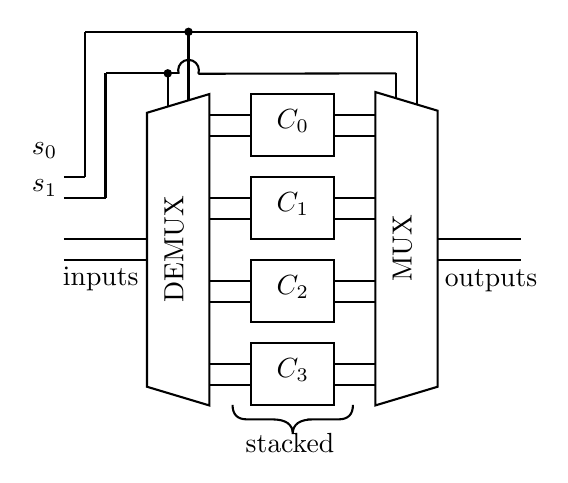
\begin{tikzpicture}[x=0.75pt,y=0.75pt,yscale=-1,xscale=1]
%uncomment if require: \path (0,300); %set diagram left start at 0, and has height of 300

%Shape: Rectangle [id:dp048587029840014395] 
\draw   (120,40) -- (160,40) -- (160,70) -- (120,70) -- cycle ;
%Shape: Rectangle [id:dp5776713339273196] 
\draw   (120,80) -- (160,80) -- (160,110) -- (120,110) -- cycle ;
%Shape: Rectangle [id:dp6797954191886235] 
\draw   (120,120) -- (160,120) -- (160,150) -- (120,150) -- cycle ;
%Shape: Rectangle [id:dp13612273639531247] 
\draw   (120,160) -- (160,160) -- (160,190) -- (120,190) -- cycle ;
%Shape: Trapezoid [id:dp8246309150363402] 
\draw   (100,190) -- (70,181) -- (70,49) -- (100,40) -- cycle ;
%Straight Lines [id:da7525185807979242] 
\draw    (100,60) -- (120,60) ;
%Straight Lines [id:da31461604940557963] 
\draw    (100,50) -- (120,50) ;
%Straight Lines [id:da25486541008995456] 
\draw    (100,100) -- (120,100) ;
%Straight Lines [id:da0077951778335063615] 
\draw    (100,90) -- (120,90) ;
%Straight Lines [id:da2905976026522047] 
\draw    (100,140) -- (120,140) ;
%Straight Lines [id:da7452387399270697] 
\draw    (100,130) -- (120,130) ;
%Straight Lines [id:da0007664179468291898] 
\draw    (100,180) -- (120,180) ;
%Straight Lines [id:da10206153239828308] 
\draw    (100,170) -- (120,170) ;
%Straight Lines [id:da762851249257401] 
\draw    (160,60) -- (180,60) ;
%Straight Lines [id:da7906149158989283] 
\draw    (160,50) -- (180,50) ;
%Straight Lines [id:da7502678160942512] 
\draw    (160,100) -- (180,100) ;
%Straight Lines [id:da9029629905302936] 
\draw    (160,90) -- (180,90) ;
%Straight Lines [id:da3474710624597941] 
\draw    (160,140) -- (180,140) ;
%Straight Lines [id:da15085166543146156] 
\draw    (160,130) -- (180,130) ;
%Straight Lines [id:da33183615362638585] 
\draw    (160,180) -- (180,180) ;
%Straight Lines [id:da3689964414613789] 
\draw    (160,170) -- (180,170) ;
%Shape: Trapezoid [id:dp3485611043917566] 
\draw   (180,39) -- (210,48) -- (210,181) -- (180,190) -- cycle ;
%Straight Lines [id:da03742821351482728] 
\draw    (30,120) -- (70,120) ;
%Straight Lines [id:da7640218221254925] 
\draw    (30,110) -- (70,110) ;
%Straight Lines [id:da956984886166125] 
\draw    (210,120) -- (250,120) ;
%Straight Lines [id:da3748285907762332] 
\draw    (210,110) -- (250,110) ;
%Straight Lines [id:da9714588986108855] 
\draw    (30,90) -- (50,90) ;
%Straight Lines [id:da8529976703877445] 
\draw    (30,80) -- (40,80) ;
%Straight Lines [id:da30690121561733863] 
\draw    (50,30) -- (50,90) ;
%Straight Lines [id:da15914818103441886] 
\draw    (85,30) -- (50,30) ;
%Straight Lines [id:da11238885987153702] 
\draw    (80,30) -- (80,46) ;
%Straight Lines [id:da3144505075089207] 
\draw    (40,10) -- (40,80) ;
%Straight Lines [id:da8817997683520893] 
\draw    (200,10) -- (40,10) ;
%Straight Lines [id:da4268960799866157] 
\draw    (90,43) -- (90,10) ;
%Shape: Arc [id:dp9375967782263986] 
\draw  [draw opacity=0] (85.3,30.21) .. controls (85.11,29.68) and (85,29.1) .. (85,28.5) .. controls (85,25.74) and (87.24,23.5) .. (90,23.5) .. controls (92.76,23.5) and (95,25.74) .. (95,28.5) .. controls (95,29.1) and (94.89,29.68) .. (94.7,30.21) -- (90,28.5) -- cycle ; \draw   (85.3,30.21) .. controls (85.11,29.68) and (85,29.1) .. (85,28.5) .. controls (85,25.74) and (87.24,23.5) .. (90,23.5) .. controls (92.76,23.5) and (95,25.74) .. (95,28.5) .. controls (95,29.1) and (94.89,29.68) .. (94.7,30.21) ;
%Straight Lines [id:da20395268049972604] 
\draw    (190,30) -- (94.7,30.21) ;
%Straight Lines [id:da9984121684679509] 
\draw    (190,42) -- (190,30) ;
%Straight Lines [id:da8655654304921162] 
\draw    (200,45) -- (200,10) ;
%Shape: Circle [id:dp15675574970767925] 
\draw  [fill={rgb, 255:red, 0; green, 0; blue, 0 }  ,fill opacity=1 ] (78.5,30) .. controls (78.5,29.17) and (79.17,28.5) .. (80,28.5) .. controls (80.83,28.5) and (81.5,29.17) .. (81.5,30) .. controls (81.5,30.83) and (80.83,31.5) .. (80,31.5) .. controls (79.17,31.5) and (78.5,30.83) .. (78.5,30) -- cycle ;
%Shape: Circle [id:dp007756137419556719] 
\draw  [fill={rgb, 255:red, 0; green, 0; blue, 0 }  ,fill opacity=1 ] (88.5,10) .. controls (88.5,9.17) and (89.17,8.5) .. (90,8.5) .. controls (90.83,8.5) and (91.5,9.17) .. (91.5,10) .. controls (91.5,10.83) and (90.83,11.5) .. (90,11.5) .. controls (89.17,11.5) and (88.5,10.83) .. (88.5,10) -- cycle ;
%Shape: Brace [id:dp3366641720684751] 
\draw   (111.21,189.72) .. controls (111.21,194.39) and (113.54,196.72) .. (118.21,196.72) -- (130.21,196.72) .. controls (136.88,196.72) and (140.21,199.05) .. (140.21,203.72) .. controls (140.21,199.05) and (143.54,196.72) .. (150.21,196.72)(147.21,196.72) -- (162.21,196.72) .. controls (166.88,196.72) and (169.21,194.39) .. (169.21,189.72) ;

% Text Node
\draw (131,45.93) node [anchor=north west][inner sep=0.75pt]   [align=left] {$\displaystyle C_{0}$};
% Text Node
\draw (131,85.93) node [anchor=north west][inner sep=0.75pt]   [align=left] {$\displaystyle C_{1}$};
% Text Node
\draw (131,125.93) node [anchor=north west][inner sep=0.75pt]   [align=left] {$\displaystyle C_{2}$};
% Text Node
\draw (131,165.93) node [anchor=north west][inner sep=0.75pt]   [align=left] {$\displaystyle C_{3}$};
% Text Node
\draw (13,61.93) node [anchor=north west][inner sep=0.75pt]   [align=left] {$\displaystyle s_{0}$};
% Text Node
\draw (13,79.93) node [anchor=north west][inner sep=0.75pt]   [align=left] {$\displaystyle s_{1}$};
% Text Node
\draw (76.93,142) node [anchor=north west][inner sep=0.75pt]  [rotate=-270] [align=left] {DEMUX};
% Text Node
\draw (186.93,132) node [anchor=north west][inner sep=0.75pt]  [rotate=-270] [align=left] {MUX};
% Text Node
\draw (28,121.93) node [anchor=north west][inner sep=0.75pt]   [align=left] {inputs};
% Text Node
\draw (212,122.93) node [anchor=north west][inner sep=0.75pt]   [align=left] {outputs};
% Text Node
\draw (116,201.93) node [anchor=north west][inner sep=0.75pt]   [align=left] {stacked};


\end{tikzpicture}


  \caption{%
    The vectorized stacking of four circuits.
    The evaluator pays only linear cost to evaluate all four branches,
    but the generator pays quadratic cost in the number of branches.
  }\label{fig:vector}
\end{figure*}

\begin{figure*}[t]
  \centering
  

\tikzset{every picture/.style={line width=0.75pt}} %set default line width to 0.75pt        

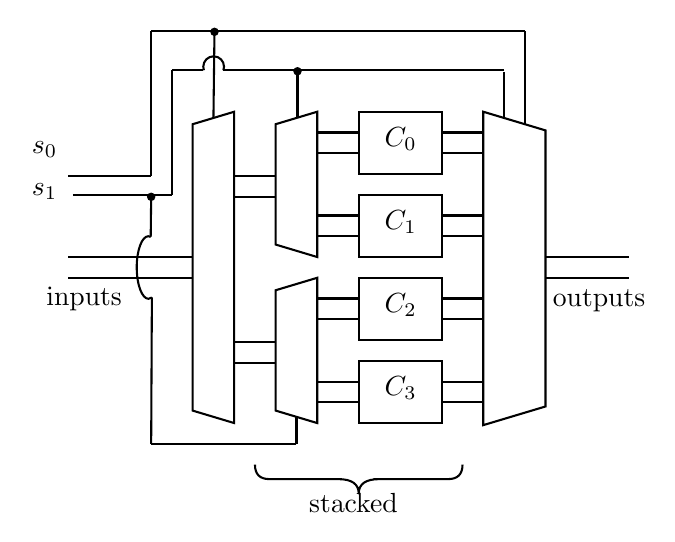
\begin{tikzpicture}[x=0.75pt,y=0.75pt,yscale=-1,xscale=1]
%uncomment if require: \path (0,300); %set diagram left start at 0, and has height of 300

%Shape: Rectangle [id:dp7502614750914376] 
\draw   (330,70) -- (370,70) -- (370,100) -- (330,100) -- cycle ;
%Shape: Rectangle [id:dp7892095271383508] 
\draw   (330,110) -- (370,110) -- (370,140) -- (330,140) -- cycle ;
%Shape: Rectangle [id:dp37989812087032515] 
\draw   (330,150) -- (370,150) -- (370,180) -- (330,180) -- cycle ;
%Shape: Rectangle [id:dp8447591317033223] 
\draw   (330,190) -- (370,190) -- (370,220) -- (330,220) -- cycle ;
%Shape: Trapezoid [id:dp7771424519284856] 
\draw   (310,140) -- (290,134) -- (290,76) -- (310,70) -- cycle ;
%Straight Lines [id:da40802590861909493] 
\draw    (310,90) -- (330,90) ;
%Straight Lines [id:da0031513249223092954] 
\draw    (310,80) -- (330,80) ;
%Straight Lines [id:da1966346673154652] 
\draw    (310,130) -- (330,130) ;
%Straight Lines [id:da6775587210008136] 
\draw    (310,120) -- (330,120) ;
%Straight Lines [id:da12476780588871761] 
\draw    (310,170) -- (330,170) ;
%Straight Lines [id:da9491489855937013] 
\draw    (310,160) -- (330,160) ;
%Straight Lines [id:da6623212585189078] 
\draw    (310,210) -- (330,210) ;
%Straight Lines [id:da6648228335361426] 
\draw    (310,200) -- (330,200) ;
%Straight Lines [id:da31517601583694976] 
\draw    (370,90) -- (390,90) ;
%Straight Lines [id:da6109875647488371] 
\draw    (370,80) -- (390,80) ;
%Straight Lines [id:da2903769623535476] 
\draw    (370,130) -- (390,130) ;
%Straight Lines [id:da8132090709679021] 
\draw    (370,120) -- (390,120) ;
%Straight Lines [id:da013751964941568051] 
\draw    (370,170) -- (390,170) ;
%Straight Lines [id:da6136724266425235] 
\draw    (370,160) -- (390,160) ;
%Straight Lines [id:da7543906971257488] 
\draw    (370,210) -- (390,210) ;
%Straight Lines [id:da5716941479183147] 
\draw    (370,200) -- (390,200) ;
%Shape: Trapezoid [id:dp7120836027835779] 
\draw   (390,70) -- (420,79) -- (420,212) -- (390,221) -- cycle ;
%Straight Lines [id:da01879494240947388] 
\draw    (190,150) -- (250,150) ;
%Straight Lines [id:da3304230275195208] 
\draw    (190,140) -- (250,140) ;
%Straight Lines [id:da1589324558664057] 
\draw    (420,150) -- (460,150) ;
%Straight Lines [id:da07702618181652965] 
\draw    (420,140) -- (460,140) ;
%Straight Lines [id:da6019545366973683] 
\draw    (192.3,110) -- (240,110) ;
%Straight Lines [id:da052523258101502934] 
\draw    (190,101) -- (230,101) ;
%Straight Lines [id:da10206301164150533] 
\draw    (260,73) -- (260.5,31.5) ;
%Shape: Trapezoid [id:dp5014208697738474] 
\draw   (310,220) -- (290,214) -- (290,156) -- (310,150) -- cycle ;
%Shape: Trapezoid [id:dp0033451661221245432] 
\draw   (270,220) -- (250,214) -- (250,76) -- (270,70) -- cycle ;
%Straight Lines [id:da6917927216058005] 
\draw    (270,111) -- (290,111) ;
%Straight Lines [id:da44243639909608434] 
\draw    (270,101) -- (290,101) ;
%Straight Lines [id:da48193219658000075] 
\draw    (270,191) -- (290,191) ;
%Straight Lines [id:da17896325371154065] 
\draw    (270,181) -- (290,181) ;
%Straight Lines [id:da693911481564593] 
\draw    (230,31) -- (230,101) ;
%Straight Lines [id:da6506643552967423] 
\draw    (410,31) -- (230,31) ;
%Straight Lines [id:da8713257514230749] 
\draw    (410,76) -- (410,31) ;
%Straight Lines [id:da3595596964731239] 
\draw    (240,50) -- (240,110) ;
%Straight Lines [id:da23325573067210137] 
\draw    (255,50) -- (240,50) ;
%Shape: Arc [id:dp43363746138961945] 
\draw  [draw opacity=0] (255.4,50) .. controls (255.21,49.47) and (255.1,48.89) .. (255.1,48.29) .. controls (255.1,45.53) and (257.34,43.29) .. (260.1,43.29) .. controls (262.86,43.29) and (265.1,45.53) .. (265.1,48.29) .. controls (265.1,48.89) and (264.99,49.47) .. (264.8,50) -- (260.1,48.29) -- cycle ; \draw   (255.4,50) .. controls (255.21,49.47) and (255.1,48.89) .. (255.1,48.29) .. controls (255.1,45.53) and (257.34,43.29) .. (260.1,43.29) .. controls (262.86,43.29) and (265.1,45.53) .. (265.1,48.29) .. controls (265.1,48.89) and (264.99,49.47) .. (264.8,50) ;
%Straight Lines [id:da664339624976211] 
\draw    (400,50) -- (264.8,50) ;
%Straight Lines [id:da8087120147451838] 
\draw    (400,73) -- (400,51) ;
%Straight Lines [id:da400002248946426] 
\draw    (300,230) -- (300,217) ;
%Straight Lines [id:da5824042733318846] 
\draw    (300,230) -- (230,230) ;
%Straight Lines [id:da44616987205982805] 
\draw    (230,111) -- (229.77,130.29) ;
%Shape: Arc [id:dp23272127004968368] 
\draw  [draw opacity=0] (230.34,159.49) .. controls (229.83,159.91) and (229.28,160.13) .. (228.72,160.13) .. controls (225.61,160.14) and (223.07,153.4) .. (223.04,145.07) .. controls (223.02,136.75) and (225.52,129.99) .. (228.64,129.98) .. controls (229.03,129.98) and (229.41,130.09) .. (229.77,130.29) -- (228.68,145.06) -- cycle ; \draw   (230.34,159.49) .. controls (229.83,159.91) and (229.28,160.13) .. (228.72,160.13) .. controls (225.61,160.14) and (223.07,153.4) .. (223.04,145.07) .. controls (223.02,136.75) and (225.52,129.99) .. (228.64,129.98) .. controls (229.03,129.98) and (229.41,130.09) .. (229.77,130.29) ;
%Straight Lines [id:da9791876678321777] 
\draw    (230.34,159.49) -- (230,230) ;
%Shape: Circle [id:dp034644651933813386] 
\draw  [fill={rgb, 255:red, 0; green, 0; blue, 0 }  ,fill opacity=1 ] (228.5,111) .. controls (228.5,110.17) and (229.17,109.5) .. (230,109.5) .. controls (230.83,109.5) and (231.5,110.17) .. (231.5,111) .. controls (231.5,111.83) and (230.83,112.5) .. (230,112.5) .. controls (229.17,112.5) and (228.5,111.83) .. (228.5,111) -- cycle ;
%Shape: Circle [id:dp9201679931345544] 
\draw  [fill={rgb, 255:red, 0; green, 0; blue, 0 }  ,fill opacity=1 ] (299,50.5) .. controls (299,49.67) and (299.67,49) .. (300.5,49) .. controls (301.33,49) and (302,49.67) .. (302,50.5) .. controls (302,51.33) and (301.33,52) .. (300.5,52) .. controls (299.67,52) and (299,51.33) .. (299,50.5) -- cycle ;
%Straight Lines [id:da30693031106532875] 
\draw    (300.5,73) -- (300.5,52) ;
%Shape: Circle [id:dp5158540745153025] 
\draw  [fill={rgb, 255:red, 0; green, 0; blue, 0 }  ,fill opacity=1 ] (259,31.5) .. controls (259,30.67) and (259.67,30) .. (260.5,30) .. controls (261.33,30) and (262,30.67) .. (262,31.5) .. controls (262,32.33) and (261.33,33) .. (260.5,33) .. controls (259.67,33) and (259,32.33) .. (259,31.5) -- cycle ;
%Shape: Brace [id:dp7057588613218542] 
\draw   (280,240) .. controls (280,244.67) and (282.33,247) .. (287,247) -- (320,247) .. controls (326.67,247) and (330,249.33) .. (330,254) .. controls (330,249.33) and (333.33,247) .. (340,247)(337,247) -- (373,247) .. controls (377.67,247) and (380,244.67) .. (380,240) ;

% Text Node
\draw (341,75.93) node [anchor=north west][inner sep=0.75pt]   [align=left] {$\displaystyle C_{0}$};
% Text Node
\draw (341,115.93) node [anchor=north west][inner sep=0.75pt]   [align=left] {$\displaystyle C_{1}$};
% Text Node
\draw (341,155.93) node [anchor=north west][inner sep=0.75pt]   [align=left] {$\displaystyle C_{2}$};
% Text Node
\draw (341,195.93) node [anchor=north west][inner sep=0.75pt]   [align=left] {$\displaystyle C_{3}$};
% Text Node
\draw (178,152.93) node [anchor=north west][inner sep=0.75pt]   [align=left] {inputs};
% Text Node
\draw (422,153.93) node [anchor=north west][inner sep=0.75pt]   [align=left] {outputs};
% Text Node
\draw (171,82.93) node [anchor=north west][inner sep=0.75pt]   [align=left] {$\displaystyle s_{0}$};
% Text Node
\draw (171,102.93) node [anchor=north west][inner sep=0.75pt]   [align=left] {$\displaystyle s_{1}$};
% Text Node
\draw (304.63,252.21) node [anchor=north west][inner sep=0.75pt]   [align=left] {stacked};


\end{tikzpicture}


  \caption{%
    Our stacking optimization.
    The four conditional branches are stacked by nesting, but the
    multiplexer is not stacked.
    By leaving the multiplexer unstacked, we prevent the players from
    recursively emulating themselves at quadratic cost.
  }\label{fig:optimized}
\end{figure*}


\begin{figure*}[t]
  \centering
  

\tikzset{every picture/.style={line width=0.75pt}} %set default line width to 0.75pt        

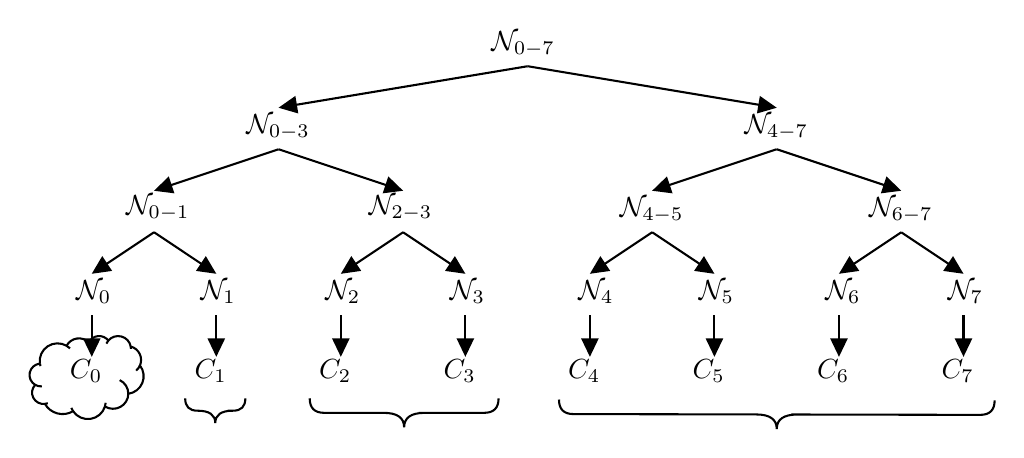
\begin{tikzpicture}[x=0.75pt,y=0.75pt,yscale=-1,xscale=1]
%uncomment if require: \path (0,300); %set diagram left start at 0, and has height of 300

%Straight Lines [id:da6211885505100274] 
\draw    (112.5,168.34) -- (140,150) ;
\draw [shift={(110,170)}, rotate = 326.31] [fill={rgb, 255:red, 0; green, 0; blue, 0 }  ][line width=0.08]  [draw opacity=0] (8.93,-4.29) -- (0,0) -- (8.93,4.29) -- cycle    ;
%Straight Lines [id:da045344571187413196] 
\draw    (140,150) -- (167.5,168.34) ;
\draw [shift={(170,170)}, rotate = 213.69] [fill={rgb, 255:red, 0; green, 0; blue, 0 }  ][line width=0.08]  [draw opacity=0] (8.93,-4.29) -- (0,0) -- (8.93,4.29) -- cycle    ;
%Straight Lines [id:da30999351200098524] 
\draw    (232.5,168.34) -- (260,150) ;
\draw [shift={(230,170)}, rotate = 326.31] [fill={rgb, 255:red, 0; green, 0; blue, 0 }  ][line width=0.08]  [draw opacity=0] (8.93,-4.29) -- (0,0) -- (8.93,4.29) -- cycle    ;
%Straight Lines [id:da0038108532391990524] 
\draw    (260,150) -- (287.5,168.34) ;
\draw [shift={(290,170)}, rotate = 213.69] [fill={rgb, 255:red, 0; green, 0; blue, 0 }  ][line width=0.08]  [draw opacity=0] (8.93,-4.29) -- (0,0) -- (8.93,4.29) -- cycle    ;
%Straight Lines [id:da5202996112606035] 
\draw    (352.5,168.34) -- (380,150) ;
\draw [shift={(350,170)}, rotate = 326.31] [fill={rgb, 255:red, 0; green, 0; blue, 0 }  ][line width=0.08]  [draw opacity=0] (8.93,-4.29) -- (0,0) -- (8.93,4.29) -- cycle    ;
%Straight Lines [id:da44817423034007153] 
\draw    (380,150) -- (407.5,168.34) ;
\draw [shift={(410,170)}, rotate = 213.69] [fill={rgb, 255:red, 0; green, 0; blue, 0 }  ][line width=0.08]  [draw opacity=0] (8.93,-4.29) -- (0,0) -- (8.93,4.29) -- cycle    ;
%Straight Lines [id:da1464427855443573] 
\draw    (472.5,168.34) -- (500,150) ;
\draw [shift={(470,170)}, rotate = 326.31] [fill={rgb, 255:red, 0; green, 0; blue, 0 }  ][line width=0.08]  [draw opacity=0] (8.93,-4.29) -- (0,0) -- (8.93,4.29) -- cycle    ;
%Straight Lines [id:da13582204926626829] 
\draw    (500,150) -- (527.5,168.34) ;
\draw [shift={(530,170)}, rotate = 213.69] [fill={rgb, 255:red, 0; green, 0; blue, 0 }  ][line width=0.08]  [draw opacity=0] (8.93,-4.29) -- (0,0) -- (8.93,4.29) -- cycle    ;
%Straight Lines [id:da30615324718513515] 
\draw    (142.85,129.05) -- (200,110) ;
\draw [shift={(140,130)}, rotate = 341.57] [fill={rgb, 255:red, 0; green, 0; blue, 0 }  ][line width=0.08]  [draw opacity=0] (8.93,-4.29) -- (0,0) -- (8.93,4.29) -- cycle    ;
%Straight Lines [id:da9271896843303857] 
\draw    (200,110) -- (257.15,129.05) ;
\draw [shift={(260,130)}, rotate = 198.43] [fill={rgb, 255:red, 0; green, 0; blue, 0 }  ][line width=0.08]  [draw opacity=0] (8.93,-4.29) -- (0,0) -- (8.93,4.29) -- cycle    ;
%Straight Lines [id:da09808697408042522] 
\draw    (382.85,129.05) -- (440,110) ;
\draw [shift={(380,130)}, rotate = 341.57] [fill={rgb, 255:red, 0; green, 0; blue, 0 }  ][line width=0.08]  [draw opacity=0] (8.93,-4.29) -- (0,0) -- (8.93,4.29) -- cycle    ;
%Straight Lines [id:da8331015133818496] 
\draw    (440,110) -- (497.15,129.05) ;
\draw [shift={(500,130)}, rotate = 198.43] [fill={rgb, 255:red, 0; green, 0; blue, 0 }  ][line width=0.08]  [draw opacity=0] (8.93,-4.29) -- (0,0) -- (8.93,4.29) -- cycle    ;
%Straight Lines [id:da898168093393371] 
\draw    (202.96,89.51) -- (320,70) ;
\draw [shift={(200,90)}, rotate = 350.54] [fill={rgb, 255:red, 0; green, 0; blue, 0 }  ][line width=0.08]  [draw opacity=0] (8.93,-4.29) -- (0,0) -- (8.93,4.29) -- cycle    ;
%Straight Lines [id:da13345957320943236] 
\draw    (320,70) -- (437.04,89.51) ;
\draw [shift={(440,90)}, rotate = 189.46] [fill={rgb, 255:red, 0; green, 0; blue, 0 }  ][line width=0.08]  [draw opacity=0] (8.93,-4.29) -- (0,0) -- (8.93,4.29) -- cycle    ;
%Straight Lines [id:da05876416812491858] 
\draw    (110,207) -- (110,190) ;
\draw [shift={(110,210)}, rotate = 270] [fill={rgb, 255:red, 0; green, 0; blue, 0 }  ][line width=0.08]  [draw opacity=0] (8.93,-4.29) -- (0,0) -- (8.93,4.29) -- cycle    ;
%Straight Lines [id:da5654275867640988] 
\draw    (170,207) -- (170,190) ;
\draw [shift={(170,210)}, rotate = 270] [fill={rgb, 255:red, 0; green, 0; blue, 0 }  ][line width=0.08]  [draw opacity=0] (8.93,-4.29) -- (0,0) -- (8.93,4.29) -- cycle    ;
%Straight Lines [id:da31932671168937365] 
\draw    (230,207) -- (230,190) ;
\draw [shift={(230,210)}, rotate = 270] [fill={rgb, 255:red, 0; green, 0; blue, 0 }  ][line width=0.08]  [draw opacity=0] (8.93,-4.29) -- (0,0) -- (8.93,4.29) -- cycle    ;
%Straight Lines [id:da11489740917816627] 
\draw    (290,207) -- (290,190) ;
\draw [shift={(290,210)}, rotate = 270] [fill={rgb, 255:red, 0; green, 0; blue, 0 }  ][line width=0.08]  [draw opacity=0] (8.93,-4.29) -- (0,0) -- (8.93,4.29) -- cycle    ;
%Straight Lines [id:da24817292659767398] 
\draw    (350,207) -- (350,190) ;
\draw [shift={(350,210)}, rotate = 270] [fill={rgb, 255:red, 0; green, 0; blue, 0 }  ][line width=0.08]  [draw opacity=0] (8.93,-4.29) -- (0,0) -- (8.93,4.29) -- cycle    ;
%Straight Lines [id:da5549995270865108] 
\draw    (410,207) -- (410,190) ;
\draw [shift={(410,210)}, rotate = 270] [fill={rgb, 255:red, 0; green, 0; blue, 0 }  ][line width=0.08]  [draw opacity=0] (8.93,-4.29) -- (0,0) -- (8.93,4.29) -- cycle    ;
%Straight Lines [id:da25264418335124195] 
\draw    (470,207) -- (470,190) ;
\draw [shift={(470,210)}, rotate = 270] [fill={rgb, 255:red, 0; green, 0; blue, 0 }  ][line width=0.08]  [draw opacity=0] (8.93,-4.29) -- (0,0) -- (8.93,4.29) -- cycle    ;
%Straight Lines [id:da07214105669651583] 
\draw    (530,207) -- (530,190) ;
\draw [shift={(530,210)}, rotate = 270] [fill={rgb, 255:red, 0; green, 0; blue, 0 }  ][line width=0.08]  [draw opacity=0] (8.93,-4.29) -- (0,0) -- (8.93,4.29) -- cycle    ;
%Shape: Cloud [id:dp5196949234271024] 
\draw   (85.01,213.17) .. controls (84.56,209.94) and (86.02,206.75) .. (88.75,204.95) .. controls (91.48,203.14) and (95.02,203.04) .. (97.85,204.68) .. controls (98.86,202.81) and (100.7,201.51) .. (102.81,201.19) .. controls (104.93,200.87) and (107.07,201.56) .. (108.6,203.05) .. controls (109.45,201.35) and (111.13,200.2) .. (113.04,200.02) .. controls (114.95,199.85) and (116.82,200.66) .. (117.98,202.17) .. controls (119.52,200.36) and (121.98,199.6) .. (124.29,200.22) .. controls (126.6,200.83) and (128.34,202.71) .. (128.77,205.03) .. controls (130.66,205.54) and (132.24,206.84) .. (133.09,208.6) .. controls (133.95,210.35) and (133.99,212.39) .. (133.22,214.18) .. controls (135.08,216.58) and (135.52,219.79) .. (134.36,222.6) .. controls (133.21,225.4) and (130.64,227.39) .. (127.61,227.82) .. controls (127.58,230.46) and (126.12,232.88) .. (123.79,234.15) .. controls (121.46,235.42) and (118.61,235.34) .. (116.35,233.94) .. controls (115.39,237.1) and (112.68,239.42) .. (109.4,239.91) .. controls (106.12,240.39) and (102.85,238.95) .. (101,236.21) .. controls (98.74,237.56) and (96.03,237.95) .. (93.47,237.29) .. controls (90.92,236.63) and (88.74,234.97) .. (87.43,232.7) .. controls (85.12,232.97) and (82.88,231.78) .. (81.83,229.73) .. controls (80.78,227.68) and (81.14,225.19) .. (82.73,223.52) .. controls (80.67,222.31) and (79.62,219.93) .. (80.13,217.6) .. controls (80.63,215.28) and (82.58,213.54) .. (84.96,213.29) ; \draw   (82.73,223.52) .. controls (83.71,224.08) and (84.83,224.34) .. (85.95,224.25)(87.43,232.7) .. controls (87.91,232.64) and (88.38,232.52) .. (88.84,232.35)(101,236.21) .. controls (100.66,235.71) and (100.38,235.16) .. (100.15,234.6)(116.35,233.94) .. controls (116.53,233.37) and (116.64,232.77) .. (116.69,232.17)(127.6,227.82) .. controls (127.63,225.02) and (126.02,222.45) .. (123.47,221.22)(133.22,214.18) .. controls (132.8,215.13) and (132.17,215.98) .. (131.38,216.66)(128.77,205.03) .. controls (128.84,205.42) and (128.87,205.81) .. (128.86,206.2)(117.98,202.17) .. controls (117.59,202.62) and (117.28,203.12) .. (117.04,203.66)(108.6,203.05) .. controls (108.39,203.45) and (108.24,203.89) .. (108.14,204.33)(97.85,204.68) .. controls (98.45,205.03) and (99.01,205.45) .. (99.51,205.93)(85.01,213.17) .. controls (85.07,213.61) and (85.16,214.05) .. (85.29,214.48) ;
%Shape: Brace [id:dp37789584804120313] 
\draw   (335.1,230.59) .. controls (335.09,235.26) and (337.41,237.59) .. (342.08,237.6) -- (430.03,237.77) .. controls (436.7,237.78) and (440.03,240.12) .. (440.02,244.79) .. controls (440.03,240.12) and (443.36,237.8) .. (450.03,237.81)(447.03,237.8) -- (537.99,237.98) .. controls (542.66,237.99) and (544.99,235.66) .. (545,230.99) ;
%Shape: Brace [id:dp3826911569900966] 
\draw   (215,230) .. controls (215,234.67) and (217.33,237) .. (222,237) -- (250.5,237) .. controls (257.17,237) and (260.5,239.33) .. (260.5,244) .. controls (260.5,239.33) and (263.83,237) .. (270.5,237)(267.5,237) -- (299,237) .. controls (303.67,237) and (306,234.67) .. (306,230) ;
%Shape: Brace [id:dp8696613256451281] 
\draw   (155,230) .. controls (155,233.98) and (156.99,235.97) .. (160.97,235.97) -- (160.97,235.97) .. controls (166.66,235.97) and (169.5,237.96) .. (169.5,241.94) .. controls (169.5,237.96) and (172.34,235.97) .. (178.03,235.97)(175.47,235.97) -- (178.03,235.97) .. controls (182.01,235.97) and (184,233.98) .. (184,230) ;

% Text Node
\draw (98,209.93) node [anchor=north west][inner sep=0.75pt]   [align=left] {$\displaystyle C_{0}$};
% Text Node
\draw (218,209.93) node [anchor=north west][inner sep=0.75pt]   [align=left] {$\displaystyle C_{2}$};
% Text Node
\draw (278,209.93) node [anchor=north west][inner sep=0.75pt]   [align=left] {$\displaystyle C_{3}$};
% Text Node
\draw (338,209.93) node [anchor=north west][inner sep=0.75pt]   [align=left] {$\displaystyle C_{4}$};
% Text Node
\draw (398,209.93) node [anchor=north west][inner sep=0.75pt]   [align=left] {$\displaystyle C_{5}$};
% Text Node
\draw (458,209.93) node [anchor=north west][inner sep=0.75pt]   [align=left] {$\displaystyle C_{6}$};
% Text Node
\draw (518,209.93) node [anchor=north west][inner sep=0.75pt]   [align=left] {$\displaystyle C_{7}$};
% Text Node
\draw (101,171.93) node [anchor=north west][inner sep=0.75pt]   [align=left] {$\displaystyle \mathcal{N}_{0}$};
% Text Node
\draw (161,171.93) node [anchor=north west][inner sep=0.75pt]   [align=left] {$\displaystyle \mathcal{N}_{1}$};
% Text Node
\draw (221,171.93) node [anchor=north west][inner sep=0.75pt]   [align=left] {$\displaystyle \mathcal{N}_{2}$};
% Text Node
\draw (281,171.93) node [anchor=north west][inner sep=0.75pt]   [align=left] {$\displaystyle \mathcal{N}_{3}$};
% Text Node
\draw (343,171.93) node [anchor=north west][inner sep=0.75pt]   [align=left] {$\displaystyle \mathcal{N}_{4}$};
% Text Node
\draw (401,171.93) node [anchor=north west][inner sep=0.75pt]   [align=left] {$\displaystyle \mathcal{N}_{5}$};
% Text Node
\draw (462,171.93) node [anchor=north west][inner sep=0.75pt]   [align=left] {$\displaystyle \mathcal{N}_{6}$};
% Text Node
\draw (521,171.93) node [anchor=north west][inner sep=0.75pt]   [align=left] {$\displaystyle \mathcal{N}_{7}$};
% Text Node
\draw (125,130.93) node [anchor=north west][inner sep=0.75pt]   [align=left] {$\displaystyle \mathcal{N}_{0-1}$};
% Text Node
\draw (242,130.93) node [anchor=north west][inner sep=0.75pt]   [align=left] {$\displaystyle \mathcal{N}_{2-3}$};
% Text Node
\draw (363,131.93) node [anchor=north west][inner sep=0.75pt]   [align=left] {$\displaystyle \mathcal{N}_{4-5}$};
% Text Node
\draw (483,131.93) node [anchor=north west][inner sep=0.75pt]   [align=left] {$\displaystyle \mathcal{N}_{6-7}$};
% Text Node
\draw (183,91.93) node [anchor=north west][inner sep=0.75pt]   [align=left] {$\displaystyle \mathcal{N}_{0-3}$};
% Text Node
\draw (423,91.93) node [anchor=north west][inner sep=0.75pt]   [align=left] {$\displaystyle \mathcal{N}_{4-7}$};
% Text Node
\draw (301,51.93) node [anchor=north west][inner sep=0.75pt]   [align=left] {$\displaystyle \mathcal{N}_{0-7}$};
% Text Node
\draw (158,209.93) node [anchor=north west][inner sep=0.75pt]   [align=left] {$\displaystyle C_{1}$};


\end{tikzpicture}


  \caption{%
    Suppose there are $8$ branches $\cir_0$ through $\cir_7$, and
    suppose \E guesses that $\cir_0$ is the taken branch.
    If the taken branch is in the subtree $\cir_4$ through $\cir_7$,
    \E will generate the same garbage material for the entire subtree,
    regardless of which branch is actually taken.
    By extension, $\cir_0$ can only be evaluated against $\log 8 = 3$ garbage
    material strings: one for each sibling subtree (sibling subtrees
    are bracketed).
  }\label{seed-tree}
\end{figure*}


\begin{itemize}
  \item Present in formal detail.
\end{itemize}

\begin{construction}\label{cnstr:ourapproach}
  \ourapproach~is something or other.
  Probably an algorithm(s).
\end{construction}
